\begin{figure}[t!]%
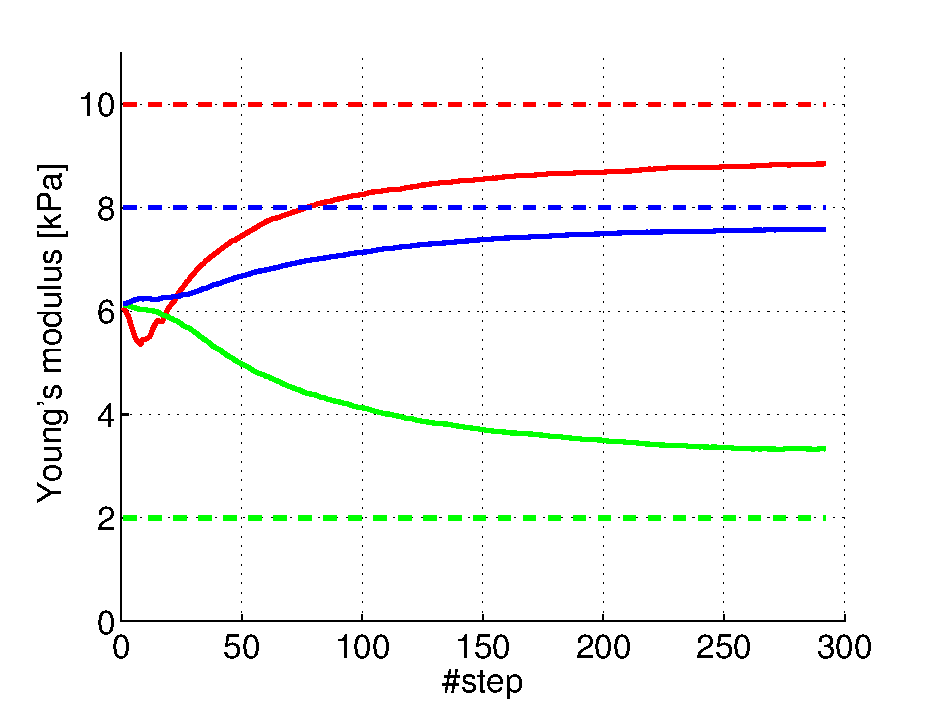
\includegraphics[height=6cm]{figs/cyl3EA_means.pdf}
\caption{The evolution of the average elastic modules computed as the mean over the element belonging to segment 1 (blue), 2 (green) and 3 (red), 
\ie\ each curve represent a mean of curves plotted in Fig.~\ref{f:cyl3EAsegs} (a), (b) and (c), respectively.}
\label{f:cyl3EAmeans}
\end{figure}

\section{Conclusion and Perspectives}
\label{s:conclusion}
In this paper, we have demonstrated that it is possible to bridge the gap between the world of physically-based models 
and the domain of data assimilation methods based on Kalman filtering. We have employed a state-of-the-art  
\emph{reduced-order unscented Kalman filter} to estimate the Young's modulus in heterogeneous object modeled by 
the co-rotational formulation of non-linear elasticity. 
%The method was based on integration of two 
%packages, SOFA and Verdandi, which was in turn employed in different scenarios as described in section~\ref{sr:scenarios}. 
We have performed an experimental estimation of system with 770 parameters; although the approach requires further 
evaluation, the preliminary results are encouraging as they suggest significant reliability and robustness of the estimator. 

We are aware of the fact that the method was evaluated using only the synthetic data which where moreover generated using 
the FE model identical to the one used in the estimation.
At the same time, we believe that the initial testing requires knowledge of the ground-truth which is
usually available only for synthetic data. 

%As the next step, we want to focus on the correction phase, so that it would allow for integration 
%of the data assimilation technique with a real-life object with known mechanical properties. 

In the near future, we plan to further improve the performance of the method. As demonstrated in section~\ref{sr:perf}, 
the parellelization of the prediction phase has brought only limited improvement, as the mathematical operations 
performed by the filter itself has become increasingly expensive, especially with growing number of parameters. 
We have already performed a code profiling in order to identify the actual bottlenecks of the algorithm. 
Since the filter manipulates mainly with the stochastic data such as the co-variance dense matrices, we have
performed a preliminary estimations showing that employing GPGPUs would resunt in a significant acceleration.
We are also working on employment of the actual version of the algorithm in real scenarios of medical planning and navigation.

\begin{figure}[t!]%
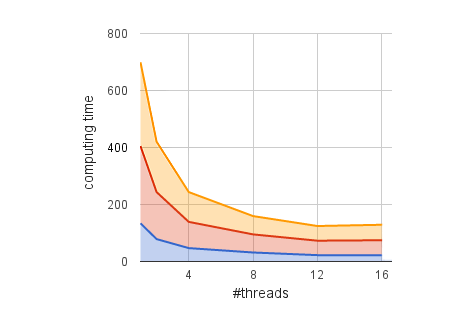
\includegraphics[height=6cm]{figs/cyl10parallel.png}
\caption{The impact of the parallelization on the computation time in [s] needed to perform 100 steps of the data assimilation used for 
the estimation of 10 parameters on mesh $\msb$. Three different types of sigma points were tested: \emph{simplex} (blue curve), 
\emph{canonical} (red curve) and \emph{star} (yellow curve).}
\label{f:parallel}
\end{figure}
